\section{Soft- und Hardware}
\label{sec:softundhardware}
%==============================================================================

Im Folgenden werden die wichtigsten Konzepte näher erläutert.

\subsection{Microsoft Kinect}
\textbf{TODO}
\begin{itemize}
  \item figure Genauigkeit in Abhängigkeit zur Entfernung
  \item Funktionsweise des PrimeSense
  \item mit Simon abstimmen
\end{itemize}

\label{subsec:kinect}

%Microsoft bietet seit November 2010 {\color{red}Quelle} ein Produkt an, das es in dieser günstigen Form zuvor nicht auf dem Markt gab: die \gls{glos:Kinect}. Die Designgrundlage stammt von einer Firma namens PrimeSense\footnote{siehe \url{http://www.primesense.com/}}, die schon seit geraumer Zeit derartige Geräte entwickelt. Eigentlich wurde das Gerät für Microsofts \gls{glos:XBOX} konzipiert, jedoch wuchs das Interesse daran stetig, als Open Source Projekte entstanden die das Protokoll über die USB-Schnittstelle zur \gls{glos:Kinect} per \gls{glos:RevEng} offenlegten. Heute wird sie in unzähligen Hobby- aber auch professionellen zu einem großen Teil universitären Projekten wie diesem eingesetzt. Dabei inspirierten die Entwickler zunächst vor allem Anwendungen bezüglich Gestensteuerung oder Skeleton Tracking wie sie auch in den Konsolenspielen eingesetzt werden. Jedoch wurde schnell ersichtlich, das das Gerät aufgrund seiner Daten in bestimmten Anwendungsfällen auch Laserscanner ersetzen und damit viele Anwendungsszenarien bedienen kann.

{\color{red}fakten:}\\

{\color{red}- aufbau (kamera, ir, ir-kamera)}\\
{\color{red}- Auflösung}\\

%Die \gls{glos:Kinect} sendet über den {\color{red}AUSFÜLLEN} ein Muster aus Infrarotpunkten aus. Wie in Abbildung \ref{fig:kinectIlluminator} zu sehen, werden diese von Objekten die im Sichtfeld des Gerätes stehen reflektiert. Gut zu erkennen ist auch, dass sich in der Szene eine flache Grundfläche und zwei senkrecht aneinander stehende leicht konvexe Flächen befinden. Aufgrund dieses Szenenaufbaus, entsteht eine ungleichmäßige Infrarotausleuchtung. Eine spezielle Software kann nun anhand der Verzerrung des Musters, dem Abstand und Größe der Infrarotlichtpunkte errechnen, in welcher Entfernung die Objekte zur Kamera stehen.
%\begin{figure}[t]
%	\centering
%	\fbox{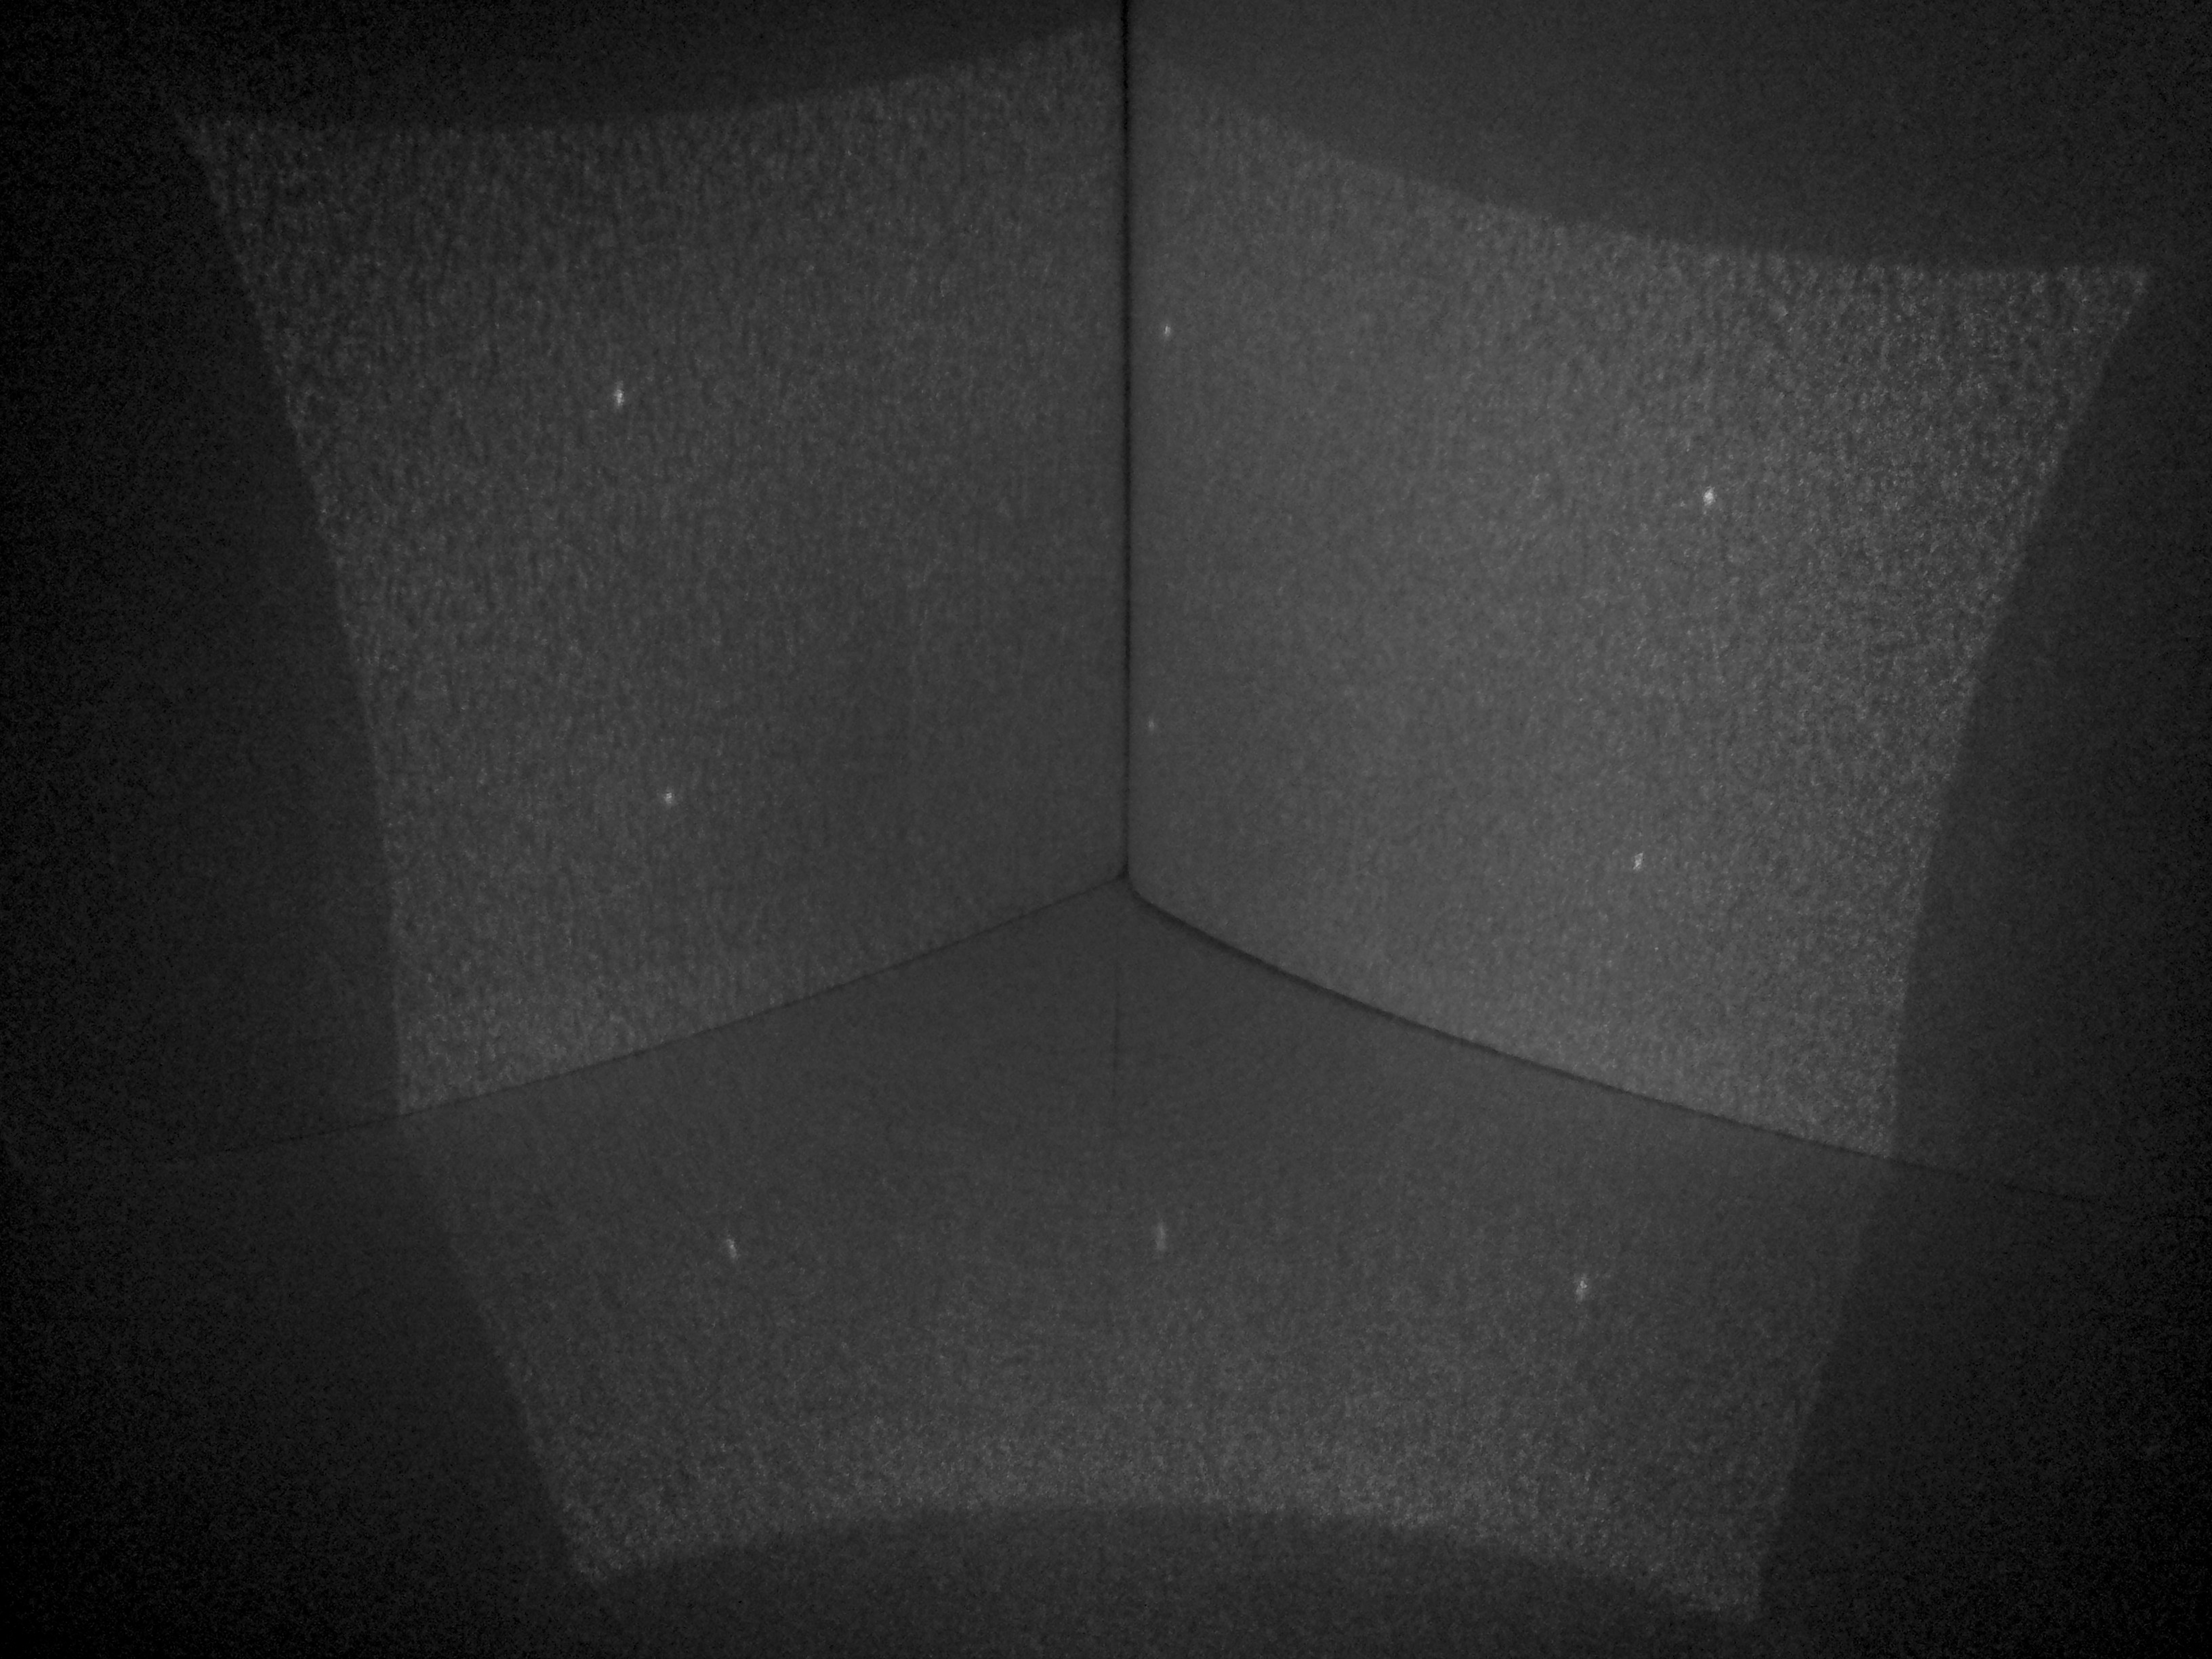
\includegraphics[height=10cm]{./graphics/kinectIlluminator_sharp2}}
%	\caption[Kinect Infrarot Feld]{Eine Aufnahme des Infrarot Ausleuchtungsfelds der \gls{glos:Kinect}.}
%	\label{fig:kinectIlluminator}
%\end{figure}
%
%Aufgrund des Aufbaus der \gls{glos:Kinect} entstehen dabei zwangsläufig tote Winkel, über die sie keine Aussagen treffen kann. Abbildung \ref{fig:toterWinkel} zeigt diesen Umstand. Das Infrarotlicht kann nicht auf die ganze hintere Wand projiziert werden, da diese von einem davor stehenden Objekt verdeckt wird. Der {\color{red}rote} Bereich liegt jedoch im Sichtfeld der Infrarotkamera. Die Abbildung \ref{fig:kinectViews} in Kapitel \ref{subsec:opennistack} zeigt diesen Effekt ebenfalls. Jedoch ist dort der Winkel des linken 3D-Bildes leicht verschoben, sodass tote Winkel scheinbar links und rechts von Objekten auftreten können. Dies ist aber wie in Abbildung \ref{fig:toterWinkel} gezeigt aufgrund des Aufbaus der \gls{glos:Kinect} nicht der Fall.
%\begin{figure}[t]
%	\centering
%	\fbox{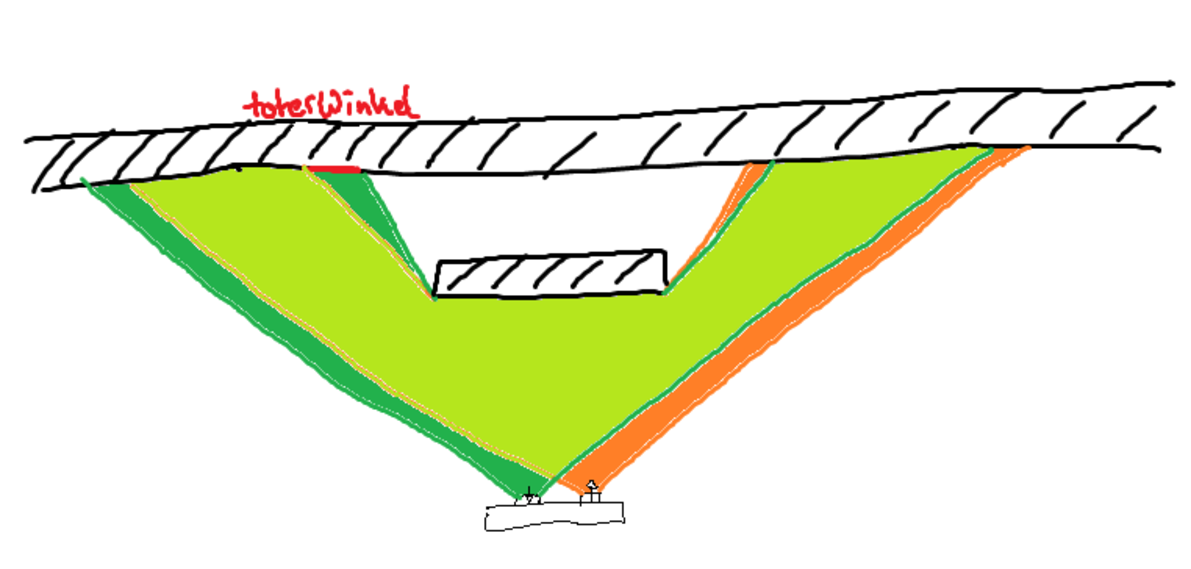
\includegraphics[height=6cm]{./graphics/toterWinkel}}
%	\caption[Toter Winkel der Kinect]{Eine anschauliche Darstellung eines toten Winkels der \gls{glos:Kinect}.}
%	\label{fig:toterWinkel}
%\end{figure}
%
%{\color{red}- Reichweite}\\
%{\color{red}- Genauigkeit in Abhängigkeit zur Entfernung (kurvenbild: kinect/optimal-linien)}\\
%{\color{red}- vergleich mit laser (kinect ca. 80 EUR, laser ca. 1500 EUR)}\\
%
%{\color{red}
%benutzungsmöglichkeiten für uns:\\
%- libfreenect, (inoffizielle api)\\
%- openni (offizielle api)\\
%- openni\_kinect stack erwähnen/referenzieren! (benutzt offizielle api)\\
%}
%
\subsection{Robot Operating System}
\begin{itemize}
  \item grundlegendes Prinzip und Aufbau
  \begin{itemize}
    \item Stacks
    \item Nodes
    \item inter Node-Kommunikation per Messages via Topics
  \end{itemize}
\end{itemize}

\subsection{rgbdslam}

